
% Default to the notebook output style

    


% Inherit from the specified cell style.




    
\documentclass[11pt]{article}

    
    
    \usepackage[T1]{fontenc}
    % Nicer default font (+ math font) than Computer Modern for most use cases
    \usepackage{mathpazo}

    % Basic figure setup, for now with no caption control since it's done
    % automatically by Pandoc (which extracts ![](path) syntax from Markdown).
    \usepackage{graphicx}
    % We will generate all images so they have a width \maxwidth. This means
    % that they will get their normal width if they fit onto the page, but
    % are scaled down if they would overflow the margins.
    \makeatletter
    \def\maxwidth{\ifdim\Gin@nat@width>\linewidth\linewidth
    \else\Gin@nat@width\fi}
    \makeatother
    \let\Oldincludegraphics\includegraphics
    % Set max figure width to be 80% of text width, for now hardcoded.
    \renewcommand{\includegraphics}[1]{\Oldincludegraphics[width=.8\maxwidth]{#1}}
    % Ensure that by default, figures have no caption (until we provide a
    % proper Figure object with a Caption API and a way to capture that
    % in the conversion process - todo).
    \usepackage{caption}
    \DeclareCaptionLabelFormat{nolabel}{}
    \captionsetup{labelformat=nolabel}

    \usepackage{adjustbox} % Used to constrain images to a maximum size 
    \usepackage{xcolor} % Allow colors to be defined
    \usepackage{enumerate} % Needed for markdown enumerations to work
    \usepackage{geometry} % Used to adjust the document margins
    \usepackage{amsmath} % Equations
    \usepackage{amssymb} % Equations
    \usepackage{textcomp} % defines textquotesingle
    % Hack from http://tex.stackexchange.com/a/47451/13684:
    \AtBeginDocument{%
        \def\PYZsq{\textquotesingle}% Upright quotes in Pygmentized code
    }
    \usepackage{upquote} % Upright quotes for verbatim code
    \usepackage{eurosym} % defines \euro
    \usepackage[mathletters]{ucs} % Extended unicode (utf-8) support
    \usepackage[utf8x]{inputenc} % Allow utf-8 characters in the tex document
    \usepackage{fancyvrb} % verbatim replacement that allows latex
    \usepackage{grffile} % extends the file name processing of package graphics 
                         % to support a larger range 
    % The hyperref package gives us a pdf with properly built
    % internal navigation ('pdf bookmarks' for the table of contents,
    % internal cross-reference links, web links for URLs, etc.)
    \usepackage{hyperref}
    \usepackage{longtable} % longtable support required by pandoc >1.10
    \usepackage{booktabs}  % table support for pandoc > 1.12.2
    \usepackage[inline]{enumitem} % IRkernel/repr support (it uses the enumerate* environment)
    \usepackage[normalem]{ulem} % ulem is needed to support strikethroughs (\sout)
                                % normalem makes italics be italics, not underlines
    

    
    
    % Colors for the hyperref package
    \definecolor{urlcolor}{rgb}{0,.145,.698}
    \definecolor{linkcolor}{rgb}{.71,0.21,0.01}
    \definecolor{citecolor}{rgb}{.12,.54,.11}

    % ANSI colors
    \definecolor{ansi-black}{HTML}{3E424D}
    \definecolor{ansi-black-intense}{HTML}{282C36}
    \definecolor{ansi-red}{HTML}{E75C58}
    \definecolor{ansi-red-intense}{HTML}{B22B31}
    \definecolor{ansi-green}{HTML}{00A250}
    \definecolor{ansi-green-intense}{HTML}{007427}
    \definecolor{ansi-yellow}{HTML}{DDB62B}
    \definecolor{ansi-yellow-intense}{HTML}{B27D12}
    \definecolor{ansi-blue}{HTML}{208FFB}
    \definecolor{ansi-blue-intense}{HTML}{0065CA}
    \definecolor{ansi-magenta}{HTML}{D160C4}
    \definecolor{ansi-magenta-intense}{HTML}{A03196}
    \definecolor{ansi-cyan}{HTML}{60C6C8}
    \definecolor{ansi-cyan-intense}{HTML}{258F8F}
    \definecolor{ansi-white}{HTML}{C5C1B4}
    \definecolor{ansi-white-intense}{HTML}{A1A6B2}

    % commands and environments needed by pandoc snippets
    % extracted from the output of `pandoc -s`
    \providecommand{\tightlist}{%
      \setlength{\itemsep}{0pt}\setlength{\parskip}{0pt}}
    \DefineVerbatimEnvironment{Highlighting}{Verbatim}{commandchars=\\\{\}}
    % Add ',fontsize=\small' for more characters per line
    \newenvironment{Shaded}{}{}
    \newcommand{\KeywordTok}[1]{\textcolor[rgb]{0.00,0.44,0.13}{\textbf{{#1}}}}
    \newcommand{\DataTypeTok}[1]{\textcolor[rgb]{0.56,0.13,0.00}{{#1}}}
    \newcommand{\DecValTok}[1]{\textcolor[rgb]{0.25,0.63,0.44}{{#1}}}
    \newcommand{\BaseNTok}[1]{\textcolor[rgb]{0.25,0.63,0.44}{{#1}}}
    \newcommand{\FloatTok}[1]{\textcolor[rgb]{0.25,0.63,0.44}{{#1}}}
    \newcommand{\CharTok}[1]{\textcolor[rgb]{0.25,0.44,0.63}{{#1}}}
    \newcommand{\StringTok}[1]{\textcolor[rgb]{0.25,0.44,0.63}{{#1}}}
    \newcommand{\CommentTok}[1]{\textcolor[rgb]{0.38,0.63,0.69}{\textit{{#1}}}}
    \newcommand{\OtherTok}[1]{\textcolor[rgb]{0.00,0.44,0.13}{{#1}}}
    \newcommand{\AlertTok}[1]{\textcolor[rgb]{1.00,0.00,0.00}{\textbf{{#1}}}}
    \newcommand{\FunctionTok}[1]{\textcolor[rgb]{0.02,0.16,0.49}{{#1}}}
    \newcommand{\RegionMarkerTok}[1]{{#1}}
    \newcommand{\ErrorTok}[1]{\textcolor[rgb]{1.00,0.00,0.00}{\textbf{{#1}}}}
    \newcommand{\NormalTok}[1]{{#1}}
    
    % Additional commands for more recent versions of Pandoc
    \newcommand{\ConstantTok}[1]{\textcolor[rgb]{0.53,0.00,0.00}{{#1}}}
    \newcommand{\SpecialCharTok}[1]{\textcolor[rgb]{0.25,0.44,0.63}{{#1}}}
    \newcommand{\VerbatimStringTok}[1]{\textcolor[rgb]{0.25,0.44,0.63}{{#1}}}
    \newcommand{\SpecialStringTok}[1]{\textcolor[rgb]{0.73,0.40,0.53}{{#1}}}
    \newcommand{\ImportTok}[1]{{#1}}
    \newcommand{\DocumentationTok}[1]{\textcolor[rgb]{0.73,0.13,0.13}{\textit{{#1}}}}
    \newcommand{\AnnotationTok}[1]{\textcolor[rgb]{0.38,0.63,0.69}{\textbf{\textit{{#1}}}}}
    \newcommand{\CommentVarTok}[1]{\textcolor[rgb]{0.38,0.63,0.69}{\textbf{\textit{{#1}}}}}
    \newcommand{\VariableTok}[1]{\textcolor[rgb]{0.10,0.09,0.49}{{#1}}}
    \newcommand{\ControlFlowTok}[1]{\textcolor[rgb]{0.00,0.44,0.13}{\textbf{{#1}}}}
    \newcommand{\OperatorTok}[1]{\textcolor[rgb]{0.40,0.40,0.40}{{#1}}}
    \newcommand{\BuiltInTok}[1]{{#1}}
    \newcommand{\ExtensionTok}[1]{{#1}}
    \newcommand{\PreprocessorTok}[1]{\textcolor[rgb]{0.74,0.48,0.00}{{#1}}}
    \newcommand{\AttributeTok}[1]{\textcolor[rgb]{0.49,0.56,0.16}{{#1}}}
    \newcommand{\InformationTok}[1]{\textcolor[rgb]{0.38,0.63,0.69}{\textbf{\textit{{#1}}}}}
    \newcommand{\WarningTok}[1]{\textcolor[rgb]{0.38,0.63,0.69}{\textbf{\textit{{#1}}}}}
    
    
    % Define a nice break command that doesn't care if a line doesn't already
    % exist.
    \def\br{\hspace*{\fill} \\* }
    % Math Jax compatability definitions
    \def\gt{>}
    \def\lt{<}
    % Document parameters
    \title{Tutorial\_Session6}
    
    
    

    % Pygments definitions
    
\makeatletter
\def\PY@reset{\let\PY@it=\relax \let\PY@bf=\relax%
    \let\PY@ul=\relax \let\PY@tc=\relax%
    \let\PY@bc=\relax \let\PY@ff=\relax}
\def\PY@tok#1{\csname PY@tok@#1\endcsname}
\def\PY@toks#1+{\ifx\relax#1\empty\else%
    \PY@tok{#1}\expandafter\PY@toks\fi}
\def\PY@do#1{\PY@bc{\PY@tc{\PY@ul{%
    \PY@it{\PY@bf{\PY@ff{#1}}}}}}}
\def\PY#1#2{\PY@reset\PY@toks#1+\relax+\PY@do{#2}}

\expandafter\def\csname PY@tok@w\endcsname{\def\PY@tc##1{\textcolor[rgb]{0.73,0.73,0.73}{##1}}}
\expandafter\def\csname PY@tok@c\endcsname{\let\PY@it=\textit\def\PY@tc##1{\textcolor[rgb]{0.25,0.50,0.50}{##1}}}
\expandafter\def\csname PY@tok@cp\endcsname{\def\PY@tc##1{\textcolor[rgb]{0.74,0.48,0.00}{##1}}}
\expandafter\def\csname PY@tok@k\endcsname{\let\PY@bf=\textbf\def\PY@tc##1{\textcolor[rgb]{0.00,0.50,0.00}{##1}}}
\expandafter\def\csname PY@tok@kp\endcsname{\def\PY@tc##1{\textcolor[rgb]{0.00,0.50,0.00}{##1}}}
\expandafter\def\csname PY@tok@kt\endcsname{\def\PY@tc##1{\textcolor[rgb]{0.69,0.00,0.25}{##1}}}
\expandafter\def\csname PY@tok@o\endcsname{\def\PY@tc##1{\textcolor[rgb]{0.40,0.40,0.40}{##1}}}
\expandafter\def\csname PY@tok@ow\endcsname{\let\PY@bf=\textbf\def\PY@tc##1{\textcolor[rgb]{0.67,0.13,1.00}{##1}}}
\expandafter\def\csname PY@tok@nb\endcsname{\def\PY@tc##1{\textcolor[rgb]{0.00,0.50,0.00}{##1}}}
\expandafter\def\csname PY@tok@nf\endcsname{\def\PY@tc##1{\textcolor[rgb]{0.00,0.00,1.00}{##1}}}
\expandafter\def\csname PY@tok@nc\endcsname{\let\PY@bf=\textbf\def\PY@tc##1{\textcolor[rgb]{0.00,0.00,1.00}{##1}}}
\expandafter\def\csname PY@tok@nn\endcsname{\let\PY@bf=\textbf\def\PY@tc##1{\textcolor[rgb]{0.00,0.00,1.00}{##1}}}
\expandafter\def\csname PY@tok@ne\endcsname{\let\PY@bf=\textbf\def\PY@tc##1{\textcolor[rgb]{0.82,0.25,0.23}{##1}}}
\expandafter\def\csname PY@tok@nv\endcsname{\def\PY@tc##1{\textcolor[rgb]{0.10,0.09,0.49}{##1}}}
\expandafter\def\csname PY@tok@no\endcsname{\def\PY@tc##1{\textcolor[rgb]{0.53,0.00,0.00}{##1}}}
\expandafter\def\csname PY@tok@nl\endcsname{\def\PY@tc##1{\textcolor[rgb]{0.63,0.63,0.00}{##1}}}
\expandafter\def\csname PY@tok@ni\endcsname{\let\PY@bf=\textbf\def\PY@tc##1{\textcolor[rgb]{0.60,0.60,0.60}{##1}}}
\expandafter\def\csname PY@tok@na\endcsname{\def\PY@tc##1{\textcolor[rgb]{0.49,0.56,0.16}{##1}}}
\expandafter\def\csname PY@tok@nt\endcsname{\let\PY@bf=\textbf\def\PY@tc##1{\textcolor[rgb]{0.00,0.50,0.00}{##1}}}
\expandafter\def\csname PY@tok@nd\endcsname{\def\PY@tc##1{\textcolor[rgb]{0.67,0.13,1.00}{##1}}}
\expandafter\def\csname PY@tok@s\endcsname{\def\PY@tc##1{\textcolor[rgb]{0.73,0.13,0.13}{##1}}}
\expandafter\def\csname PY@tok@sd\endcsname{\let\PY@it=\textit\def\PY@tc##1{\textcolor[rgb]{0.73,0.13,0.13}{##1}}}
\expandafter\def\csname PY@tok@si\endcsname{\let\PY@bf=\textbf\def\PY@tc##1{\textcolor[rgb]{0.73,0.40,0.53}{##1}}}
\expandafter\def\csname PY@tok@se\endcsname{\let\PY@bf=\textbf\def\PY@tc##1{\textcolor[rgb]{0.73,0.40,0.13}{##1}}}
\expandafter\def\csname PY@tok@sr\endcsname{\def\PY@tc##1{\textcolor[rgb]{0.73,0.40,0.53}{##1}}}
\expandafter\def\csname PY@tok@ss\endcsname{\def\PY@tc##1{\textcolor[rgb]{0.10,0.09,0.49}{##1}}}
\expandafter\def\csname PY@tok@sx\endcsname{\def\PY@tc##1{\textcolor[rgb]{0.00,0.50,0.00}{##1}}}
\expandafter\def\csname PY@tok@m\endcsname{\def\PY@tc##1{\textcolor[rgb]{0.40,0.40,0.40}{##1}}}
\expandafter\def\csname PY@tok@gh\endcsname{\let\PY@bf=\textbf\def\PY@tc##1{\textcolor[rgb]{0.00,0.00,0.50}{##1}}}
\expandafter\def\csname PY@tok@gu\endcsname{\let\PY@bf=\textbf\def\PY@tc##1{\textcolor[rgb]{0.50,0.00,0.50}{##1}}}
\expandafter\def\csname PY@tok@gd\endcsname{\def\PY@tc##1{\textcolor[rgb]{0.63,0.00,0.00}{##1}}}
\expandafter\def\csname PY@tok@gi\endcsname{\def\PY@tc##1{\textcolor[rgb]{0.00,0.63,0.00}{##1}}}
\expandafter\def\csname PY@tok@gr\endcsname{\def\PY@tc##1{\textcolor[rgb]{1.00,0.00,0.00}{##1}}}
\expandafter\def\csname PY@tok@ge\endcsname{\let\PY@it=\textit}
\expandafter\def\csname PY@tok@gs\endcsname{\let\PY@bf=\textbf}
\expandafter\def\csname PY@tok@gp\endcsname{\let\PY@bf=\textbf\def\PY@tc##1{\textcolor[rgb]{0.00,0.00,0.50}{##1}}}
\expandafter\def\csname PY@tok@go\endcsname{\def\PY@tc##1{\textcolor[rgb]{0.53,0.53,0.53}{##1}}}
\expandafter\def\csname PY@tok@gt\endcsname{\def\PY@tc##1{\textcolor[rgb]{0.00,0.27,0.87}{##1}}}
\expandafter\def\csname PY@tok@err\endcsname{\def\PY@bc##1{\setlength{\fboxsep}{0pt}\fcolorbox[rgb]{1.00,0.00,0.00}{1,1,1}{\strut ##1}}}
\expandafter\def\csname PY@tok@kc\endcsname{\let\PY@bf=\textbf\def\PY@tc##1{\textcolor[rgb]{0.00,0.50,0.00}{##1}}}
\expandafter\def\csname PY@tok@kd\endcsname{\let\PY@bf=\textbf\def\PY@tc##1{\textcolor[rgb]{0.00,0.50,0.00}{##1}}}
\expandafter\def\csname PY@tok@kn\endcsname{\let\PY@bf=\textbf\def\PY@tc##1{\textcolor[rgb]{0.00,0.50,0.00}{##1}}}
\expandafter\def\csname PY@tok@kr\endcsname{\let\PY@bf=\textbf\def\PY@tc##1{\textcolor[rgb]{0.00,0.50,0.00}{##1}}}
\expandafter\def\csname PY@tok@bp\endcsname{\def\PY@tc##1{\textcolor[rgb]{0.00,0.50,0.00}{##1}}}
\expandafter\def\csname PY@tok@fm\endcsname{\def\PY@tc##1{\textcolor[rgb]{0.00,0.00,1.00}{##1}}}
\expandafter\def\csname PY@tok@vc\endcsname{\def\PY@tc##1{\textcolor[rgb]{0.10,0.09,0.49}{##1}}}
\expandafter\def\csname PY@tok@vg\endcsname{\def\PY@tc##1{\textcolor[rgb]{0.10,0.09,0.49}{##1}}}
\expandafter\def\csname PY@tok@vi\endcsname{\def\PY@tc##1{\textcolor[rgb]{0.10,0.09,0.49}{##1}}}
\expandafter\def\csname PY@tok@vm\endcsname{\def\PY@tc##1{\textcolor[rgb]{0.10,0.09,0.49}{##1}}}
\expandafter\def\csname PY@tok@sa\endcsname{\def\PY@tc##1{\textcolor[rgb]{0.73,0.13,0.13}{##1}}}
\expandafter\def\csname PY@tok@sb\endcsname{\def\PY@tc##1{\textcolor[rgb]{0.73,0.13,0.13}{##1}}}
\expandafter\def\csname PY@tok@sc\endcsname{\def\PY@tc##1{\textcolor[rgb]{0.73,0.13,0.13}{##1}}}
\expandafter\def\csname PY@tok@dl\endcsname{\def\PY@tc##1{\textcolor[rgb]{0.73,0.13,0.13}{##1}}}
\expandafter\def\csname PY@tok@s2\endcsname{\def\PY@tc##1{\textcolor[rgb]{0.73,0.13,0.13}{##1}}}
\expandafter\def\csname PY@tok@sh\endcsname{\def\PY@tc##1{\textcolor[rgb]{0.73,0.13,0.13}{##1}}}
\expandafter\def\csname PY@tok@s1\endcsname{\def\PY@tc##1{\textcolor[rgb]{0.73,0.13,0.13}{##1}}}
\expandafter\def\csname PY@tok@mb\endcsname{\def\PY@tc##1{\textcolor[rgb]{0.40,0.40,0.40}{##1}}}
\expandafter\def\csname PY@tok@mf\endcsname{\def\PY@tc##1{\textcolor[rgb]{0.40,0.40,0.40}{##1}}}
\expandafter\def\csname PY@tok@mh\endcsname{\def\PY@tc##1{\textcolor[rgb]{0.40,0.40,0.40}{##1}}}
\expandafter\def\csname PY@tok@mi\endcsname{\def\PY@tc##1{\textcolor[rgb]{0.40,0.40,0.40}{##1}}}
\expandafter\def\csname PY@tok@il\endcsname{\def\PY@tc##1{\textcolor[rgb]{0.40,0.40,0.40}{##1}}}
\expandafter\def\csname PY@tok@mo\endcsname{\def\PY@tc##1{\textcolor[rgb]{0.40,0.40,0.40}{##1}}}
\expandafter\def\csname PY@tok@ch\endcsname{\let\PY@it=\textit\def\PY@tc##1{\textcolor[rgb]{0.25,0.50,0.50}{##1}}}
\expandafter\def\csname PY@tok@cm\endcsname{\let\PY@it=\textit\def\PY@tc##1{\textcolor[rgb]{0.25,0.50,0.50}{##1}}}
\expandafter\def\csname PY@tok@cpf\endcsname{\let\PY@it=\textit\def\PY@tc##1{\textcolor[rgb]{0.25,0.50,0.50}{##1}}}
\expandafter\def\csname PY@tok@c1\endcsname{\let\PY@it=\textit\def\PY@tc##1{\textcolor[rgb]{0.25,0.50,0.50}{##1}}}
\expandafter\def\csname PY@tok@cs\endcsname{\let\PY@it=\textit\def\PY@tc##1{\textcolor[rgb]{0.25,0.50,0.50}{##1}}}

\def\PYZbs{\char`\\}
\def\PYZus{\char`\_}
\def\PYZob{\char`\{}
\def\PYZcb{\char`\}}
\def\PYZca{\char`\^}
\def\PYZam{\char`\&}
\def\PYZlt{\char`\<}
\def\PYZgt{\char`\>}
\def\PYZsh{\char`\#}
\def\PYZpc{\char`\%}
\def\PYZdl{\char`\$}
\def\PYZhy{\char`\-}
\def\PYZsq{\char`\'}
\def\PYZdq{\char`\"}
\def\PYZti{\char`\~}
% for compatibility with earlier versions
\def\PYZat{@}
\def\PYZlb{[}
\def\PYZrb{]}
\makeatother


    % Exact colors from NB
    \definecolor{incolor}{rgb}{0.0, 0.0, 0.5}
    \definecolor{outcolor}{rgb}{0.545, 0.0, 0.0}



    
    % Prevent overflowing lines due to hard-to-break entities
    \sloppy 
    % Setup hyperref package
    \hypersetup{
      breaklinks=true,  % so long urls are correctly broken across lines
      colorlinks=true,
      urlcolor=urlcolor,
      linkcolor=linkcolor,
      citecolor=citecolor,
      }
    % Slightly bigger margins than the latex defaults
    
    \geometry{verbose,tmargin=1in,bmargin=1in,lmargin=1in,rmargin=1in}
    
    

    \begin{document}
    
    
    \maketitle
    
    

    
    \section{ CLASSES }\label{classes}

\begin{itemize}
\tightlist
\item
  A class is a template that provides a logical grouping of data and
  methods that operate on them.
\item
  Instances of a class are called objects.
\item
  Data and methods associated with a class are collectively known as
  class attributes.
\end{itemize}

    \subsection{ Classes and Objects }\label{classes-and-objects}

\begin{itemize}
\tightlist
\item
  Variables used so far took values of types (also called classes)
  string (str), integer (int), floating point (float), Boolean (bool),
  list, tuple, or dictionary (dict).
\end{itemize}

    \begin{Verbatim}[commandchars=\\\{\}]
{\color{incolor}In [{\color{incolor}3}]:} \PY{n+nb}{print}\PY{p}{(}\PY{n+nb}{type}\PY{p}{(}\PY{l+m+mi}{12}\PY{p}{)}\PY{p}{,} \PY{n+nb}{type}\PY{p}{(}\PY{l+m+mf}{12.5}\PY{p}{)}\PY{p}{,} \PY{n+nb}{type}\PY{p}{(}\PY{l+s+s1}{\PYZsq{}}\PY{l+s+s1}{hello}\PY{l+s+s1}{\PYZsq{}}\PY{p}{)}\PY{p}{)}
\end{Verbatim}


    \begin{Verbatim}[commandchars=\\\{\}]
<class 'int'> <class 'float'> <class 'str'>

    \end{Verbatim}

    ** Accessing attribute of an instance of class** * To specify an
attribute of a class (or class instance), we write the name of the class
(or class instance) followed by a dot, followed by the name of that
attribute. The method \textbf{lower} defined in class \textbf{str} has
been invoked for the object \textbf{name}.

    \begin{Verbatim}[commandchars=\\\{\}]
{\color{incolor}In [{\color{incolor}4}]:} \PY{n}{name} \PY{o}{=} \PY{l+s+s1}{\PYZsq{}}\PY{l+s+s1}{Raman}\PY{l+s+s1}{\PYZsq{}}
        \PY{n}{lname} \PY{o}{=} \PY{n}{name}\PY{o}{.}\PY{n}{lower}\PY{p}{(}\PY{p}{)}
        \PY{n+nb}{print}\PY{p}{(}\PY{n}{lname}\PY{p}{)}
\end{Verbatim}


    \begin{Verbatim}[commandchars=\\\{\}]
raman

    \end{Verbatim}

    \textbf{Alternative way of invoking the method associated with an
instance of class}: * Specify the name of the class (str), followed by
the dot operator (.), followed by the name of the method (lower),
followed by an object (name). The object name being an argument is
enclosed in parentheses.

    \begin{Verbatim}[commandchars=\\\{\}]
{\color{incolor}In [{\color{incolor}5}]:} \PY{n}{lname} \PY{o}{=} \PY{n+nb}{str}\PY{o}{.}\PY{n}{lower}\PY{p}{(}\PY{n}{name}\PY{p}{)}
        \PY{n+nb}{print}\PY{p}{(}\PY{n}{lname}\PY{p}{)}
\end{Verbatim}


    \begin{Verbatim}[commandchars=\\\{\}]
raman

    \end{Verbatim}

    \begin{center}\rule{0.5\linewidth}{\linethickness}\end{center}

\subsection{ PERSON class }\label{person-class}

\subsubsection{ Syntax of Class Definiton
}\label{syntax-of-class-definiton}

A class definition begins with the keyword class followed by the name of
the class, and a colon. By convention, the first letter of the class
name is capitalized. The syntax for class definition is as follows:

\begin{verbatim}
class ClassName:
    classBody
    
    
\end{verbatim}

\subsubsection{ Operations supported by classes:
}\label{operations-supported-by-classes}

\begin{enumerate}
\def\labelenumi{\arabic{enumi}.}
\tightlist
\item
  \textbf{Instantiation}: It refers to the creation of an object, i.e.
  an instance of the class.
\item
  \textbf{Attribute references}: Methods and data members of an object
  of a class are accessed using the notation: name of the object,
  followed by dot operator, followed by the member name.
\end{enumerate}

    \begin{Verbatim}[commandchars=\\\{\}]
{\color{incolor}In [{\color{incolor}5}]:} \PY{k}{class} \PY{n+nc}{Person}\PY{p}{:}
            \PY{l+s+sd}{\PYZsq{}\PYZsq{}\PYZsq{} The class Person describes a person\PYZsq{}\PYZsq{}\PYZsq{}}
            \PY{n}{count} \PY{o}{=} \PY{l+m+mi}{0}
            \PY{k}{def} \PY{n+nf}{\PYZus{}\PYZus{}init\PYZus{}\PYZus{}}\PY{p}{(}\PY{n+nb+bp}{self}\PY{p}{,} \PY{n}{name}\PY{p}{,} \PY{n}{DOB}\PY{p}{,} \PY{n}{address}\PY{p}{)}\PY{p}{:}
                \PY{l+s+sd}{\PYZsq{}\PYZsq{}\PYZsq{}}
        \PY{l+s+sd}{        Objective: To initialize object of class Person}
        \PY{l+s+sd}{        Input Parameters:}
        \PY{l+s+sd}{            self (implicit parameter) \PYZhy{} object of type Person}
        \PY{l+s+sd}{            name \PYZhy{} string}
        \PY{l+s+sd}{            DOB \PYZhy{} string (Date of Birth)}
        \PY{l+s+sd}{            address \PYZhy{} string}
        \PY{l+s+sd}{        Return Value: None}
        \PY{l+s+sd}{        \PYZsq{}\PYZsq{}\PYZsq{}}
                \PY{n+nb+bp}{self}\PY{o}{.}\PY{n}{name} \PY{o}{=} \PY{n}{name}
                \PY{n+nb+bp}{self}\PY{o}{.}\PY{n}{DOB} \PY{o}{=} \PY{n}{DOB}
                \PY{n+nb+bp}{self}\PY{o}{.}\PY{n}{address} \PY{o}{=} \PY{n}{address}
                \PY{n}{Person}\PY{o}{.}\PY{n}{count} \PY{o}{+}\PY{o}{=} \PY{l+m+mi}{1}
        
            \PY{k}{def} \PY{n+nf}{getName}\PY{p}{(}\PY{n+nb+bp}{self}\PY{p}{)}\PY{p}{:}
                \PY{l+s+sd}{\PYZsq{}\PYZsq{}\PYZsq{}}
        \PY{l+s+sd}{        Objective: To retrieve name of the person}
        \PY{l+s+sd}{        Input Parameter: self (implicit parameter) \PYZhy{} object of type Person}
        \PY{l+s+sd}{        Return Value: name \PYZhy{} string}
        \PY{l+s+sd}{        \PYZsq{}\PYZsq{}\PYZsq{}}
                \PY{k}{return} \PY{n+nb+bp}{self}\PY{o}{.}\PY{n}{name}
        
            \PY{k}{def} \PY{n+nf}{getDOB}\PY{p}{(}\PY{n+nb+bp}{self}\PY{p}{)}\PY{p}{:}
                \PY{l+s+sd}{\PYZsq{}\PYZsq{}\PYZsq{}}
        \PY{l+s+sd}{        Objective: To retrieve the date of birth of a person}
        \PY{l+s+sd}{        Input Parameter: self (implicit parameter) \PYZhy{} object of type Person}
        \PY{l+s+sd}{        Return Value: DOB \PYZhy{} string}
        \PY{l+s+sd}{        \PYZsq{}\PYZsq{}\PYZsq{}}
                \PY{k}{return} \PY{n+nb+bp}{self}\PY{o}{.}\PY{n}{DOB}
        
            \PY{k}{def} \PY{n+nf}{getAddress}\PY{p}{(}\PY{n+nb+bp}{self}\PY{p}{)}\PY{p}{:}
                \PY{l+s+sd}{\PYZsq{}\PYZsq{}\PYZsq{}}
        \PY{l+s+sd}{        Objective: To retrieve address of person}
        \PY{l+s+sd}{        Input Parameter: self (implicit parameter) \PYZhy{} object of type Person}
        \PY{l+s+sd}{        Return Value: address \PYZhy{} string}
        \PY{l+s+sd}{        \PYZsq{}\PYZsq{}\PYZsq{}}
                \PY{k}{return} \PY{n+nb+bp}{self}\PY{o}{.}\PY{n}{address}
        
            \PY{k}{def} \PY{n+nf}{getCount}\PY{p}{(}\PY{n+nb+bp}{self}\PY{p}{)}\PY{p}{:}
                \PY{l+s+sd}{\PYZsq{}\PYZsq{}\PYZsq{}}
        \PY{l+s+sd}{        Objective: To get count of objects of type Person}
        \PY{l+s+sd}{        Input Parameter: self (implicit parameter) \PYZhy{} object of type Person}
        \PY{l+s+sd}{        Return Value: count: numeric}
        \PY{l+s+sd}{        \PYZsq{}\PYZsq{}\PYZsq{}}
                \PY{k}{return} \PY{n}{Person}\PY{o}{.}\PY{n}{count}
        
            \PY{k}{def} \PY{n+nf}{\PYZus{}\PYZus{}str\PYZus{}\PYZus{}}\PY{p}{(}\PY{n+nb+bp}{self}\PY{p}{)}\PY{p}{:}
                \PY{l+s+sd}{\PYZsq{}\PYZsq{}\PYZsq{}}
        \PY{l+s+sd}{        Objective: To return string representation of object of type Person}
        \PY{l+s+sd}{        Input Parameter: self (implicit parameter)\PYZhy{} object of type}
        \PY{l+s+sd}{        Person}
        \PY{l+s+sd}{        Return Value: string}
        \PY{l+s+sd}{        \PYZsq{}\PYZsq{}\PYZsq{}}
                \PY{k}{return} \PY{l+s+s1}{\PYZsq{}}\PY{l+s+s1}{Name:}\PY{l+s+s1}{\PYZsq{}}\PY{o}{+}\PY{n+nb+bp}{self}\PY{o}{.}\PY{n}{name}\PY{o}{+}\PY{l+s+s1}{\PYZsq{}}\PY{l+s+se}{\PYZbs{}n}\PY{l+s+s1}{DOB:}\PY{l+s+s1}{\PYZsq{}}\PY{o}{+}\PY{n+nb}{str}\PY{p}{(}\PY{n+nb+bp}{self}\PY{o}{.}\PY{n}{DOB}\PY{p}{)}\PYZbs{}
                \PY{o}{+}\PY{l+s+s1}{\PYZsq{}}\PY{l+s+se}{\PYZbs{}n}\PY{l+s+s1}{Address:}\PY{l+s+s1}{\PYZsq{}}\PY{o}{+}\PY{n+nb+bp}{self}\PY{o}{.}\PY{n}{address}
\end{Verbatim}


    \subsubsection{ Creating an instance of class Person
}\label{creating-an-instance-of-class-person}

    \begin{Verbatim}[commandchars=\\\{\}]
{\color{incolor}In [{\color{incolor}6}]:} \PY{n}{p1} \PY{o}{=} \PY{n}{Person}\PY{p}{(}\PY{l+s+s1}{\PYZsq{}}\PY{l+s+s1}{Amir}\PY{l+s+s1}{\PYZsq{}}\PY{p}{,}\PY{l+s+s1}{\PYZsq{}}\PY{l+s+s1}{24\PYZhy{}10\PYZhy{}1990}\PY{l+s+s1}{\PYZsq{}}\PY{p}{,}\PY{l+s+s1}{\PYZsq{}}\PY{l+s+s1}{38/4, IIT Delhi 110016}\PY{l+s+s1}{\PYZsq{}}\PY{p}{)}
        \PY{n+nb}{print}\PY{p}{(}\PY{n}{Person}\PY{o}{.}\PY{n}{count}\PY{p}{)}
\end{Verbatim}


    \begin{Verbatim}[commandchars=\\\{\}]
1

    \end{Verbatim}

    The execution of the above statement does three things: 1. Creates an
instance of class Person 2. Initializes it by invoking the method
\textbf{\_\_init\_\_} defined in lines 3. Returns a reference to it, so
the name p1 now refers to the instance of the class Person that has just
been created

By default, Python passes object itself (such as p1) as the first
argument to the method \textbf{\_\_init\_\_}.

    \subsubsection{ Instance p1 of class Person
}\label{instance-p1-of-class-person}

    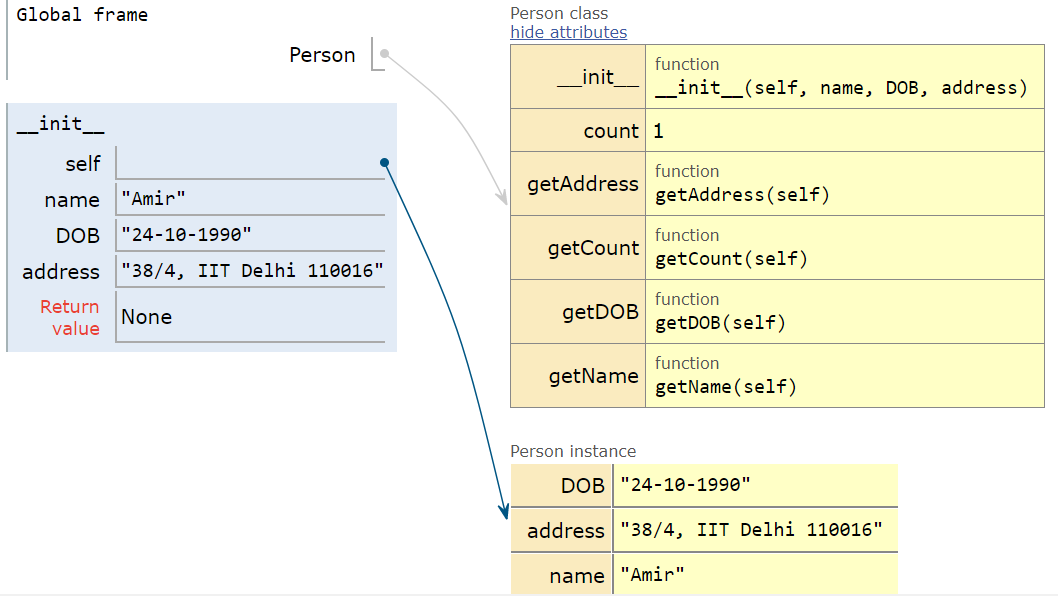
\includegraphics{1.png}

    \subsubsection{ Printing an instance of class
}\label{printing-an-instance-of-class}

Python invokes \textbf{\_\_str\_\_} method of the corresponding class to
obtain a string representation of the object

    \begin{Verbatim}[commandchars=\\\{\}]
{\color{incolor}In [{\color{incolor}61}]:} \PY{n+nb}{print}\PY{p}{(}\PY{l+m+mi}{7}\PY{p}{)}
         \PY{c+c1}{\PYZsh{} OR}
         \PY{n+nb}{print}\PY{p}{(}\PY{n+nb}{int}\PY{o}{.}\PY{n+nf+fm}{\PYZus{}\PYZus{}str\PYZus{}\PYZus{}}\PY{p}{(}\PY{l+m+mi}{7}\PY{p}{)}\PY{p}{)}
         \PY{n+nb}{print}\PY{p}{(}\PY{n+nb}{str}\PY{p}{(}\PY{l+m+mi}{7}\PY{p}{)}\PY{p}{)}
\end{Verbatim}


    \begin{Verbatim}[commandchars=\\\{\}]
7
7
7

    \end{Verbatim}

    \begin{Verbatim}[commandchars=\\\{\}]
{\color{incolor}In [{\color{incolor}151}]:} \PY{n+nb}{print}\PY{p}{(}\PY{n}{p1}\PY{p}{)}
          \PY{n+nb}{print}\PY{p}{(}\PY{l+s+s1}{\PYZsq{}}\PY{l+s+s1}{*****************}\PY{l+s+s1}{\PYZsq{}}\PY{p}{)}
          \PY{n+nb}{print}\PY{p}{(}\PY{n}{p1}\PY{o}{.}\PY{n+nf+fm}{\PYZus{}\PYZus{}str\PYZus{}\PYZus{}}\PY{p}{(}\PY{p}{)}\PY{p}{)}
          \PY{n+nb}{print}\PY{p}{(}\PY{l+s+s1}{\PYZsq{}}\PY{l+s+s1}{*****************}\PY{l+s+s1}{\PYZsq{}}\PY{p}{)}
          \PY{n+nb}{print}\PY{p}{(}\PY{n}{Person}\PY{o}{.}\PY{n+nf+fm}{\PYZus{}\PYZus{}str\PYZus{}\PYZus{}}\PY{p}{(}\PY{n}{p1}\PY{p}{)}\PY{p}{)}
          \PY{n+nb}{print}\PY{p}{(}\PY{l+s+s1}{\PYZsq{}}\PY{l+s+s1}{*****************}\PY{l+s+s1}{\PYZsq{}}\PY{p}{)}
          \PY{n+nb}{print}\PY{p}{(}\PY{n+nb}{str}\PY{p}{(}\PY{n}{p1}\PY{p}{)}\PY{p}{)}
\end{Verbatim}


    \begin{Verbatim}[commandchars=\\\{\}]
Name:Amir
DOB:24-10-1990
Address:38/4, IIT Delhi 110016
*****************
Name:Amir
DOB:24-10-1990
Address:38/4, IIT Delhi 110016
*****************
Name:Amir
DOB:24-10-1990
Address:38/4, IIT Delhi 110016
*****************
Name:Amir
DOB:24-10-1990
Address:38/4, IIT Delhi 110016

    \end{Verbatim}

    \begin{Verbatim}[commandchars=\\\{\}]
{\color{incolor}In [{\color{incolor}63}]:} \PY{n}{p1}\PY{o}{.}\PY{n}{getDOB}\PY{p}{(}\PY{p}{)}
\end{Verbatim}


\begin{Verbatim}[commandchars=\\\{\}]
{\color{outcolor}Out[{\color{outcolor}63}]:} '24-10-1990'
\end{Verbatim}
            
    \subsubsection{ List of attributes of the object
}\label{list-of-attributes-of-the-object}

    \begin{Verbatim}[commandchars=\\\{\}]
{\color{incolor}In [{\color{incolor}64}]:} \PY{n+nb}{dir}\PY{p}{(}\PY{n}{p1}\PY{p}{)}
\end{Verbatim}


\begin{Verbatim}[commandchars=\\\{\}]
{\color{outcolor}Out[{\color{outcolor}64}]:} ['DOB',
          '\_\_class\_\_',
          '\_\_delattr\_\_',
          '\_\_dict\_\_',
          '\_\_dir\_\_',
          '\_\_doc\_\_',
          '\_\_eq\_\_',
          '\_\_format\_\_',
          '\_\_ge\_\_',
          '\_\_getattribute\_\_',
          '\_\_gt\_\_',
          '\_\_hash\_\_',
          '\_\_init\_\_',
          '\_\_init\_subclass\_\_',
          '\_\_le\_\_',
          '\_\_lt\_\_',
          '\_\_module\_\_',
          '\_\_ne\_\_',
          '\_\_new\_\_',
          '\_\_reduce\_\_',
          '\_\_reduce\_ex\_\_',
          '\_\_repr\_\_',
          '\_\_setattr\_\_',
          '\_\_sizeof\_\_',
          '\_\_str\_\_',
          '\_\_subclasshook\_\_',
          '\_\_weakref\_\_',
          'address',
          'count',
          'getAddress',
          'getCount',
          'getDOB',
          'getName',
          'name']
\end{Verbatim}
            
    \subsubsection{ Deleting an object of class Person
}\label{deleting-an-object-of-class-person}

    \begin{Verbatim}[commandchars=\\\{\}]
{\color{incolor}In [{\color{incolor}7}]:} \PY{k}{def} \PY{n+nf}{\PYZus{}\PYZus{}del\PYZus{}\PYZus{}}\PY{p}{(}\PY{n+nb+bp}{self}\PY{p}{)}\PY{p}{:}
            \PY{l+s+sd}{\PYZsq{}\PYZsq{}\PYZsq{}}
        \PY{l+s+sd}{    Objective: To be invoked on deletion of an instance of the}
        \PY{l+s+sd}{    class Person}
        \PY{l+s+sd}{    Input Parameter:}
        \PY{l+s+sd}{    self (implicit parameter) – object of type Person}
        \PY{l+s+sd}{    Return Value: None}
        \PY{l+s+sd}{    \PYZsq{}\PYZsq{}\PYZsq{}}
            \PY{n+nb}{print}\PY{p}{(}\PY{l+s+s1}{\PYZsq{}}\PY{l+s+s1}{Deleted !!}\PY{l+s+s1}{\PYZsq{}}\PY{p}{)}
            \PY{n}{Person}\PY{o}{.}\PY{n}{count} \PY{o}{\PYZhy{}}\PY{o}{=} \PY{l+m+mi}{1}
\end{Verbatim}


    \begin{Verbatim}[commandchars=\\\{\}]
{\color{incolor}In [{\color{incolor}8}]:} \PY{n}{p1}\PY{o}{.}\PY{n+nf+fm}{\PYZus{}\PYZus{}del\PYZus{}\PYZus{}} \PY{o}{=} \PY{n+nf+fm}{\PYZus{}\PYZus{}del\PYZus{}\PYZus{}}
\end{Verbatim}


    \begin{Verbatim}[commandchars=\\\{\}]
{\color{incolor}In [{\color{incolor}9}]:} \PY{k}{del} \PY{n}{p1}
\end{Verbatim}


    \begin{Verbatim}[commandchars=\\\{\}]
{\color{incolor}In [{\color{incolor}10}]:} \PY{n+nb}{print}\PY{p}{(}\PY{n}{p1}\PY{p}{)}
\end{Verbatim}


    \begin{Verbatim}[commandchars=\\\{\}]

        ---------------------------------------------------------------------------

        NameError                                 Traceback (most recent call last)

        <ipython-input-10-71a0f0e933fe> in <module>()
    ----> 1 print(p1)
    

        NameError: name 'p1' is not defined

    \end{Verbatim}

    \begin{center}\rule{0.5\linewidth}{\linethickness}\end{center}

\subsection{ Inheritance }\label{inheritance}

\begin{itemize}
\tightlist
\item
  Inheritance is an important feature of object oriented programming
  that imparts ability to a class to inherit properties and behavior of
  another class

  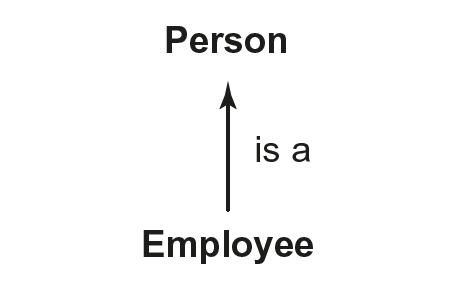
\includegraphics{2.png}
\item
  In the language of Object-oriented Programming (OOP), we say that
  Employee class inherits or derives the data and method attributes from
  the Person class.
\item
  Here, Person class is called base, super, or parent class, and
  Employee class is called derived, sub, or child class.
\end{itemize}

    \subsubsection{ Single Inheritance }\label{single-inheritance}

\begin{itemize}
\tightlist
\item
  When inheritance involves a derived class that derives its properties
  from a single base class, it is called \textbf{single inheritance}
\end{itemize}

    \begin{Verbatim}[commandchars=\\\{\}]
{\color{incolor}In [{\color{incolor}36}]:} \PY{k}{class} \PY{n+nc}{Employee}\PY{p}{(}\PY{n}{Person}\PY{p}{)}\PY{p}{:}
             \PY{n}{nextId} \PY{o}{=} \PY{l+m+mi}{1001}
             \PY{n}{empCount} \PY{o}{=} \PY{l+m+mi}{0}
         
             \PY{k}{def} \PY{n+nf}{\PYZus{}\PYZus{}init\PYZus{}\PYZus{}}\PY{p}{(}\PY{n+nb+bp}{self}\PY{p}{,} \PY{n}{name}\PY{p}{,} \PY{n}{DOB}\PY{p}{,} \PY{n}{address}\PY{p}{,} \PY{n}{basicSalary}\PY{p}{,} \PY{n}{dateOfJoining}\PY{p}{)}\PY{p}{:}
                 \PY{l+s+sd}{\PYZsq{}\PYZsq{}\PYZsq{}}
         \PY{l+s+sd}{        Objective: To initialize an object of class Employee}
         \PY{l+s+sd}{        Input Parameters:}
         \PY{l+s+sd}{            self (implicit parameter) – object of type Employee}
         \PY{l+s+sd}{            name \PYZhy{} string, address – string}
         \PY{l+s+sd}{            DOB \PYZhy{} Date of Birth – object of type MyDate}
         \PY{l+s+sd}{            basicSalary \PYZhy{} numeric value}
         \PY{l+s+sd}{            dateOfJoining – object of type MyDate}
         \PY{l+s+sd}{        Return Value: None}
         \PY{l+s+sd}{        \PYZsq{}\PYZsq{}\PYZsq{}}
                 \PY{n}{Person}\PY{o}{.}\PY{n+nf+fm}{\PYZus{}\PYZus{}init\PYZus{}\PYZus{}}\PY{p}{(}\PY{n+nb+bp}{self}\PY{p}{,} \PY{n}{name}\PY{p}{,} \PY{n}{DOB}\PY{p}{,} \PY{n}{address}\PY{p}{)}
                 \PY{n+nb+bp}{self}\PY{o}{.}\PY{n}{idNum} \PY{o}{=} \PY{n}{Employee}\PY{o}{.}\PY{n}{nextId}
                 \PY{n+nb+bp}{self}\PY{o}{.}\PY{n}{basicSalary} \PY{o}{=} \PY{n}{basicSalary}
                 \PY{n+nb+bp}{self}\PY{o}{.}\PY{n}{dateOfJoining} \PY{o}{=} \PY{n}{dateOfJoining}
                 \PY{n}{Employee}\PY{o}{.}\PY{n}{nextId} \PY{o}{+}\PY{o}{=} \PY{l+m+mi}{1}
                 \PY{n}{Employee}\PY{o}{.}\PY{n}{empCount} \PY{o}{+}\PY{o}{=} \PY{l+m+mi}{1}
         
             \PY{k}{def} \PY{n+nf}{getId}\PY{p}{(}\PY{n+nb+bp}{self}\PY{p}{)}\PY{p}{:}
                 \PY{l+s+sd}{\PYZsq{}\PYZsq{}\PYZsq{}}
         \PY{l+s+sd}{        Objective: To retrieve id of the Employee}
         \PY{l+s+sd}{        Input Parameter: self (implicit parameter)– object of type Employee}
         \PY{l+s+sd}{        Return Value: id \PYZhy{} numeric value}
         \PY{l+s+sd}{        \PYZsq{}\PYZsq{}\PYZsq{}}
                 \PY{k}{return} \PY{n+nb+bp}{self}\PY{o}{.}\PY{n}{idNum}
         
             \PY{k}{def} \PY{n+nf}{getSalary}\PY{p}{(}\PY{n+nb+bp}{self}\PY{p}{)}\PY{p}{:}
                 \PY{l+s+sd}{\PYZsq{}\PYZsq{}\PYZsq{}}
         \PY{l+s+sd}{        Objective: To retrieve salary of the Employee}
         \PY{l+s+sd}{        Input Parameter: self (implicit parameter) \PYZhy{} object of type Employee}
         \PY{l+s+sd}{        Return Value: basicSalary \PYZhy{} numeric value}
         \PY{l+s+sd}{        \PYZsq{}\PYZsq{}\PYZsq{}}
                 \PY{k}{return} \PY{n+nb+bp}{self}\PY{o}{.}\PY{n}{basicSalary}
         
             \PY{k}{def} \PY{n+nf}{reviseSalary}\PY{p}{(}\PY{n+nb+bp}{self}\PY{p}{,} \PY{n}{newSalary}\PY{p}{)}\PY{p}{:}
                 \PY{l+s+sd}{\PYZsq{}\PYZsq{}\PYZsq{}}
         \PY{l+s+sd}{        Objective: To update salary of the Employee}
         \PY{l+s+sd}{        Input Parameters: self (implicit parameter) \PYZhy{} object of type Employee}
         \PY{l+s+sd}{        newSalary \PYZhy{} numeric value}
         \PY{l+s+sd}{        Return Value: None}
         \PY{l+s+sd}{        \PYZsq{}\PYZsq{}\PYZsq{}}
                 \PY{n+nb+bp}{self}\PY{o}{.}\PY{n}{basicSalary} \PY{o}{=} \PY{n}{newSalary}
         
             \PY{k}{def} \PY{n+nf}{getJoiningDate}\PY{p}{(}\PY{n+nb+bp}{self}\PY{p}{)}\PY{p}{:}
                 \PY{l+s+sd}{\PYZsq{}\PYZsq{}\PYZsq{}}
         \PY{l+s+sd}{        Objective: To retrieve joining date of the Employee}
         \PY{l+s+sd}{        Input Parameter: self (implicit parameter) \PYZhy{} object of type Employee}
         \PY{l+s+sd}{        Return Value: dateOfJoining \PYZhy{} object of type MyDate}
         \PY{l+s+sd}{        \PYZsq{}\PYZsq{}\PYZsq{}}
                 \PY{k}{return} \PY{n+nb+bp}{self}\PY{o}{.}\PY{n}{dateOfJoining}
         
             \PY{k}{def} \PY{n+nf}{\PYZus{}\PYZus{}str\PYZus{}\PYZus{}}\PY{p}{(}\PY{n+nb+bp}{self}\PY{p}{)}\PY{p}{:}
                 \PY{l+s+sd}{\PYZsq{}\PYZsq{}\PYZsq{}}
         \PY{l+s+sd}{        Objective: To return string representation of object of type}
         \PY{l+s+sd}{        Employee.}
         \PY{l+s+sd}{        Input Parameter: self (implicit parameter) \PYZhy{} object of type Employee}
         \PY{l+s+sd}{        Return Value: string}
         \PY{l+s+sd}{        \PYZsq{}\PYZsq{}\PYZsq{}}
                 \PY{k}{return} \PY{n}{Person}\PY{o}{.}\PY{n+nf+fm}{\PYZus{}\PYZus{}str\PYZus{}\PYZus{}}\PY{p}{(}\PY{n+nb+bp}{self}\PY{p}{)}\PY{o}{+}\PY{l+s+s1}{\PYZsq{}}\PY{l+s+se}{\PYZbs{}n}\PY{l+s+s1}{Id:}\PY{l+s+s1}{\PYZsq{}}\PY{o}{+}\PY{n+nb}{str}\PY{p}{(}\PY{n+nb+bp}{self}\PY{o}{.}\PY{n}{getId}\PY{p}{(}\PY{p}{)}\PY{p}{)}\PY{o}{+}\PYZbs{}
                     \PY{l+s+s1}{\PYZsq{}}\PY{l+s+se}{\PYZbs{}n}\PY{l+s+s1}{Salary:}\PY{l+s+s1}{\PYZsq{}}\PY{o}{+}\PY{n+nb}{str}\PY{p}{(}\PY{n+nb+bp}{self}\PY{o}{.}\PY{n}{getSalary}\PY{p}{(}\PY{p}{)}\PY{p}{)}\PY{o}{+}\PYZbs{}
                     \PY{l+s+s1}{\PYZsq{}}\PY{l+s+se}{\PYZbs{}n}\PY{l+s+s1}{Date of Joining:}\PY{l+s+s1}{\PYZsq{}}\PY{o}{+}\PY{n+nb}{str}\PY{p}{(}\PY{n+nb+bp}{self}\PY{o}{.}\PY{n}{getJoiningDate}\PY{p}{(}\PY{p}{)}\PY{p}{)}
\end{Verbatim}


    \begin{Verbatim}[commandchars=\\\{\}]
{\color{incolor}In [{\color{incolor}37}]:} \PY{n}{emp1} \PY{o}{=} \PY{n}{Employee}\PY{p}{(}\PY{l+s+s1}{\PYZsq{}}\PY{l+s+s1}{Rehman}\PY{l+s+s1}{\PYZsq{}}\PY{p}{,} \PY{l+s+s1}{\PYZsq{}}\PY{l+s+s1}{5 June 1990}\PY{l+s+s1}{\PYZsq{}}\PY{p}{,} \PY{l+s+s1}{\PYZsq{}}\PY{l+s+s1}{ D\PYZhy{}9, Vivek Vihar, Delhi}\PY{l+s+s1}{\PYZsq{}}\PY{p}{,} \PY{l+m+mi}{50000}\PY{p}{,} \PY{l+s+s1}{\PYZsq{}}\PY{l+s+s1}{2 August 2013}\PY{l+s+s1}{\PYZsq{}}\PY{p}{)}
\end{Verbatim}


    \begin{Verbatim}[commandchars=\\\{\}]
{\color{incolor}In [{\color{incolor}38}]:} \PY{n+nb}{print}\PY{p}{(}\PY{n}{Employee}\PY{o}{.}\PY{n}{empCount}\PY{p}{)}
\end{Verbatim}


    \begin{Verbatim}[commandchars=\\\{\}]
1

    \end{Verbatim}

    \begin{itemize}
\item
  Call to the method \textbf{init} is made using a superclass name and
  the object instance is explicitly passed as an argument to the
  superclass method.
\item
  Alternatively, we may use the \textbf{super} function to access a
  method of the superclass.

\begin{verbatim}
super(Employee, self).__init__(name, DOB, address)
super().__init__(name, DOB, address)
\end{verbatim}
\end{itemize}

    \begin{center}\rule{0.5\linewidth}{\linethickness}\end{center}

\subsection{ 5. Built-in Functions for Classes
}\label{built-in-functions-for-classes}

    \subsubsection{ Function issubclass }\label{function-issubclass}

\begin{itemize}
\item
  The function issubclass returns True if sub is the subclass of class
  super, and False otherwise.

\begin{verbatim}
issubclass(sub, super)
\end{verbatim}
\end{itemize}

    \begin{Verbatim}[commandchars=\\\{\}]
{\color{incolor}In [{\color{incolor}146}]:} \PY{n+nb}{issubclass}\PY{p}{(}\PY{n}{Employee}\PY{p}{,} \PY{n}{Person}\PY{p}{)}
\end{Verbatim}


\begin{Verbatim}[commandchars=\\\{\}]
{\color{outcolor}Out[{\color{outcolor}146}]:} True
\end{Verbatim}
            
    \subsubsection{ Function isinstance }\label{function-isinstance}

\begin{itemize}
\item
  The function isinstance returns True if either obj is an instance of
  class class1 or it is an instance of a subclass of class class1.

\begin{verbatim}
isinstance(obj, class1)
\end{verbatim}
\end{itemize}

    \begin{Verbatim}[commandchars=\\\{\}]
{\color{incolor}In [{\color{incolor}147}]:} \PY{n+nb}{isinstance}\PY{p}{(}\PY{n}{emp1}\PY{p}{,} \PY{n}{Person}\PY{p}{)}
\end{Verbatim}


\begin{Verbatim}[commandchars=\\\{\}]
{\color{outcolor}Out[{\color{outcolor}147}]:} True
\end{Verbatim}
            
    \subsubsection{ Function hasattr }\label{function-hasattr}

\begin{itemize}
\item
  The function hasattr returns True if instance obj contains an
  attribute attr, and False otherwise.

\begin{verbatim}
hasattr(obj, attr)
\end{verbatim}
\end{itemize}

    \begin{Verbatim}[commandchars=\\\{\}]
{\color{incolor}In [{\color{incolor}149}]:} \PY{n+nb}{hasattr}\PY{p}{(}\PY{n}{emp1}\PY{p}{,} \PY{l+s+s1}{\PYZsq{}}\PY{l+s+s1}{dateOfJoining}\PY{l+s+s1}{\PYZsq{}}\PY{p}{)}
\end{Verbatim}


\begin{Verbatim}[commandchars=\\\{\}]
{\color{outcolor}Out[{\color{outcolor}149}]:} True
\end{Verbatim}
            

    % Add a bibliography block to the postdoc
    
    
    
    \end{document}
